\clearpage
\section{Programmablauf und Safety-Logik}
\label{sec:flowchart}

Abbildung~\ref{fig:flowchart} zeigt den Ablauf des Gesamtsystems. Raspberry Pi 1
übernimmt Bedienung, Anzeige, Logging und die zyklische Heartbeat-Kommunikation.
Raspberry Pi 2 führt die Sensorerfassung, Safety-Logik und Motorsteuerung aus.

\begin{figure}[H]
    \centering
    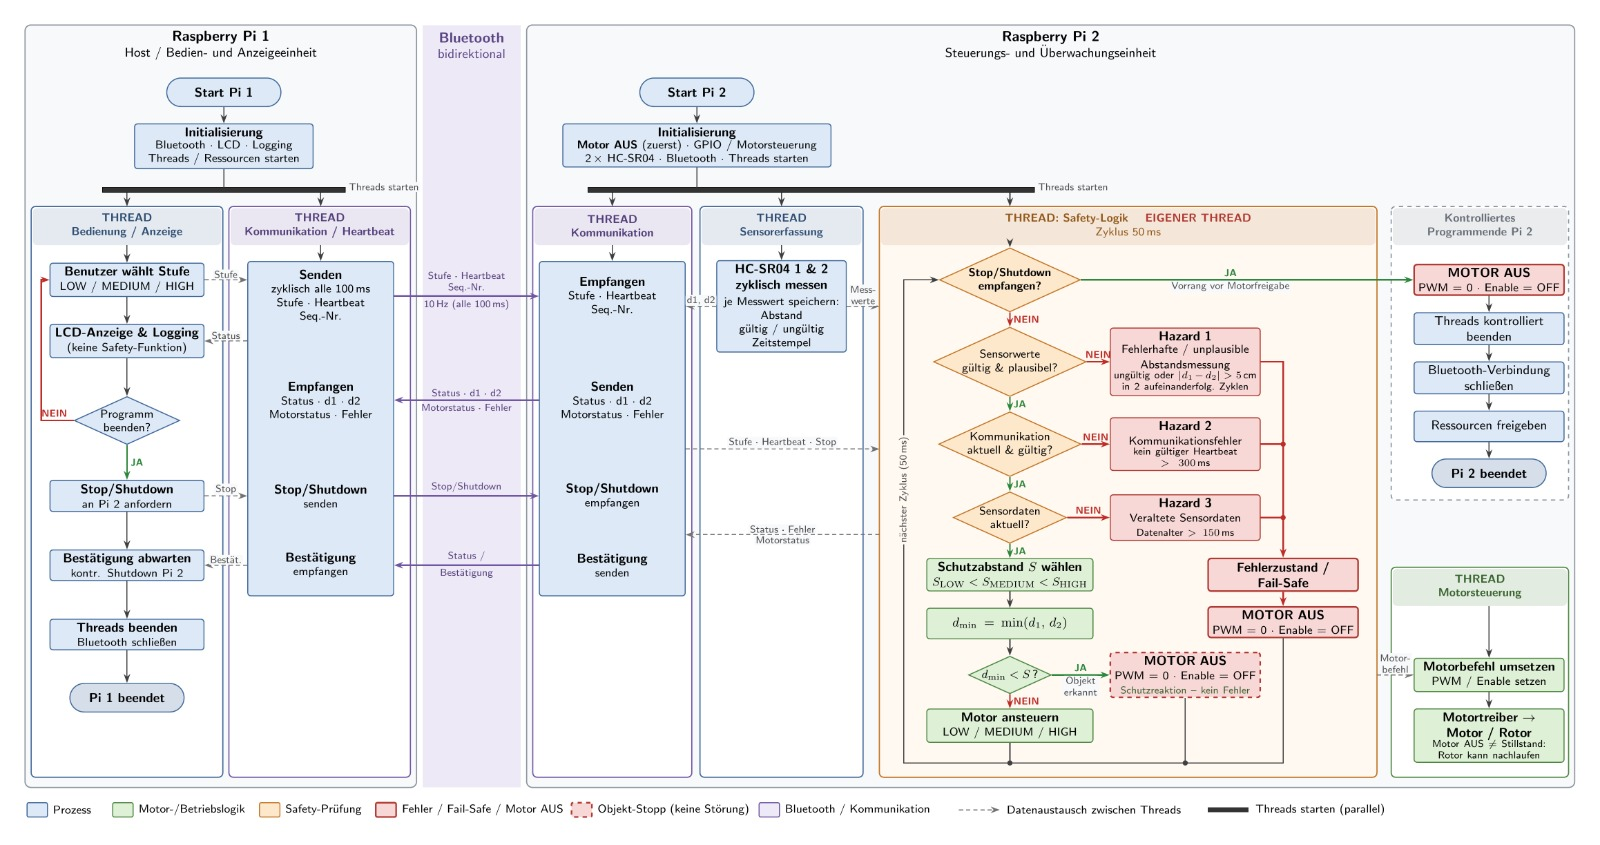
\includegraphics[width=\textwidth]{images/Campus26_Gruppe3_Flowchart_final.jpeg}
    \caption{Flussdiagramm des Gesamtsystems mit den drei adressierten Safety Hazards}
    \label{fig:flowchart}
\end{figure}

Der Safety-Logik-Thread auf Raspberry Pi 2 arbeitet zyklisch und prüft drei
Freigabebedingungen. Die Prüfungen sind logisch UND-verknüpft: Nur wenn alle drei
Bedingungen erfüllt sind, wird der Sicherheitsabstand ausgewertet und eine
Motorfreigabe ist möglich.

\begin{enumerate}
    \item \textbf{Sensorplausibilität:} Beide Sensorwerte müssen gültig sein. Eine Abweichung von mehr als 5 cm in zwei aufeinanderfolgenden Messzyklen wird als Fehler bewertet. Zusätzlich werden Messbereich und Abstandsänderung jedes Sensors geprüft (siehe Abschnitt~\ref{sec:plausibility}).
    \item \textbf{Kommunikation:} Eine gültige Nachricht bzw. ein Heartbeat muss rechtzeitig eintreffen. Bei mehr als 300 ms ohne gültige Nachricht wird der Motor abgeschaltet.
    \item \textbf{Datenaktualität:} Sensordaten dürfen höchstens 150 ms alt sein. Ältere Daten gelten als ungültig.
\end{enumerate}

Nach bestandenen Prüfungen wird der Sicherheitsabstand entsprechend der
Geschwindigkeitsstufe ausgewählt. Ist der aktuelle Abstand kleiner als der
Sicherheitsabstand, wird der Motor abgeschaltet. Andernfalls darf der Motor mit
der freigegebenen Stufe betrieben werden.

Nach jedem Zyklus beginnt die Prüfung von vorn. Fehler und Objekt-Stopp sind
daher nicht selbsthaltend: Sind im nächsten Zyklus alle Bedingungen erfüllt,
läuft der Motor ohne Quittierung wieder an (Wiederanlaufbedingung, siehe
Abschnitt~\ref{sec:states}).

Das Programmende ist ebenfalls Teil des Ablaufs. Ein Stop/Shutdown-Befehl von
Raspberry Pi 1 führt auf Raspberry Pi 2 zuerst zu Motor AUS und anschließend zum
kontrollierten Beenden des Programms.
